\documentclass{article}

\usepackage{geometry}
\usepackage{amsmath}
\usepackage{graphicx, eso-pic}
\usepackage{listings}
\usepackage{hyperref}
\usepackage{multicol}
\usepackage{fancyhdr}
\pagestyle{fancy}
\fancyhf{}
\hypersetup{ colorlinks=true, linkcolor=black, filecolor=magenta, urlcolor=cyan}
\geometry{ a4paper, total={170mm,257mm}, top=40mm, right=20mm, bottom=20mm, left=20mm}
\setlength{\parindent}{0pt}
\setlength{\parskip}{0.3em}
\renewcommand{\headrulewidth}{0pt}
\AddToShipoutPictureBG{%
  \AtPageUpperLeft{%
    \raisebox{-\height}{
\includegraphics[width=\paperwidth, height=30mm]{../headerarkav.png}}
  }
}
\rfoot{\thepage}
\lfoot{Final Competitive Programming - Arkavidia 7.0}
\lstset{
    basicstyle=\ttfamily\small,
    columns=fixed,
    extendedchars=true,
    breaklines=true,
    tabsize=2,
    prebreak=\raisebox{0ex}[0ex][0ex]{\ensuremath{\hookleftarrow}},
    frame=none,
    showtabs=false,
    showspaces=false,
    showstringspaces=false,
    prebreak={},
    keywordstyle=\color[rgb]{0.627,0.126,0.941},
    commentstyle=\color[rgb]{0.133,0.545,0.133},
    stringstyle=\color[rgb]{01,0,0},
    captionpos=t,
    escapeinside={(\%}{\%)}
}

\begin{document}

\begin{center}
    \section*{D - Daniel bermain Tetris} % ganti judul soal

    \begin{tabular}{ | c c | }
        \hline
        Batas Waktu  & 1s \\    % jangan lupa ganti time limit
        Batas Memori & 64MB \\  % jangan lupa ganti memory limit
        \hline
    \end{tabular}
\end{center}

\subsection*{Deskripsi}
Daniel sedang memainkan game Tetris. Papan Tetris tersebut memiliki lebar $N$ dan tinggi yang tidak terbatas. Seperti game Tetris pada umumnya, Daniel akan mendapatkan 1 poin jika suatu baris penuh. Daniel akan memainkan $Q$ buah game. Pada setiap game, Daniel mendapat $K$ buah trimino, yaitu potongan tetris berukuran 3. Setiap trimino dapat diubah menjadi bentuk $L$ atau $I$, dan dapat dirotasikan sebesar $90^{\circ}$ derajat beberapa kali (mungkin juga 0). Jika Daniel bermain dengan optimal, tentukan jumlah poin maksimum yang dapat dicapai. Beberapa contoh bentuk trimino yang sah adalah:

\begin{center}

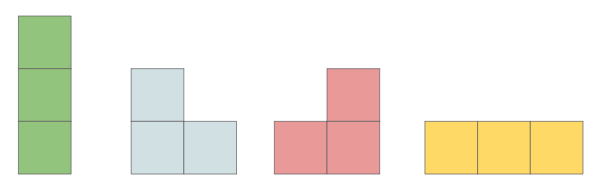
\includegraphics[scale=0.5]{possible.png}

\end{center}

\subsection*{Format Masukan}
Baris pertama berisi bilangan bulat $N$ $(1 \leq N \leq 10^9)$, menyatakan lebar papan.

Baris kedua berisi bilangan bulat $Q$ $(1 \leq Q \leq 10^5)$, menyatakan banyaknya game yang dimainkan.

$Q$ Baris berikutnya berisi bilangan bulat $K_i$ $(1 \leq K_i \leq 10^9)$ untuk setiap $i$ $(1 \leq i \leq Q)$, menyatakan banyaknya trimino yang didapatkan.

\subsection*{Format Keluaran}
Keluarkan $Q$ buah baris, dengan setiap baris merupakan jumlah poin maksimum yang dapat dicapai.

\begin{multicols}{2}
\subsection*{Contoh Masukan}
\begin{lstlisting}
3
2
1
3
\end{lstlisting}
\columnbreak
\subsection*{Contoh Keluaran}
\begin{lstlisting}
1
3
\end{lstlisting}
\vfill
\null
\end{multicols}

\subsection*{Penjelasan}

Berikut ini adalah gambar dari solusi yang mungkin:

\begin{center}

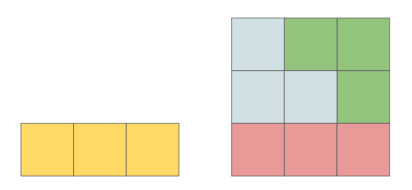
\includegraphics[scale=0.5]{answer.png}

\end{center}

\pagebreak

\end{document}